\subsection{Support Vector Machine (SVM)}

Support Vector Machine (SVM) mencari \textit{hyperplane} pemisah yang memaksimalkan
\textit{margin}, yaitu jarak terkecil antara bidang pemisah dan titik-titik data
terdekat (\textit{support vector}). Untuk data yang tidak sepenuhnya terpisah
secara linear, digunakan \textit{soft margin} dengan variabel \textit{slack}
$\xi_i \ge 0$ dan parameter regularisasi $C$:
\[
\min_{w,b,\xi}\ \frac{1}{2}\lVert w \rVert^2 + C\sum_{i=1}^n \xi_i
\quad \text{s.t.}\quad y_i(w^\top x_i + b) \ge 1 - \xi_i,\ \xi_i \ge 0 .
\]
Bentuk \textit{dual}-nya adalah
\[
\max_{\alpha}\ \sum_{i=1}^n \alpha_i
- \frac{1}{2}\sum_{i=1}^n\sum_{j=1}^n \alpha_i\alpha_j y_i y_j K(x_i,x_j),
\quad
\text{s.t.}\quad 0 \le \alpha_i \le C,\ \sum_{i=1}^n \alpha_i y_i = 0,
\]
sehingga fungsi keputusan hanya bergantung pada \textit{support vector}:
\[
f(x) = \sum_{i \in SV}\alpha_i y_i K(x_i,x) + b .
\]
\textit{Kernel trick} memungkinkan SVM memisahkan data non-linear tanpa
menghitung pemetaan fitur secara eksplisit. Pada tugas ini SVM diimplementasikan
dari nol untuk klasifikasi biner target \texttt{is\_canceled} pada dataset hotel
(27.373 baris latih, 6.844 baris uji, 32,77\% kelas positif).

\subsubsection{Implementasi}

Implementasi SVM dari nol berada pada paket \texttt{src/svm/} dan dipisahkan
menjadi empat komponen utama:
\begin{itemize}
  \item \texttt{kernels.py}: fungsi kernel \textit{linear}, \textit{polinomial},
        dan RBF, beserta resolusi nilai $\gamma$;
  \item \texttt{smo.py}: \textit{solver} Sequential Minimal Optimization (SMO)
        dengan pemilihan \textit{working set} orde kedua dan \textit{cache} kernel;
  \item \texttt{model.py}: kelas \texttt{SVM} yang menyatukan kernel, solver,
        penyimpanan \textit{support vector}, serta prediksi;
  \item \texttt{features.py} dan \texttt{data.py}: rekayasa fitur (target
        encoding, fitur interaksi, penskalaan \textit{robust}) dan pemuatan data.
\end{itemize}

\paragraph{Fungsi kernel.}
Tiga kernel yang didukung adalah kernel linear, polinomial, dan RBF
(\textit{Radial Basis Function}):
\[
K_{\text{linear}}(x,z)=x^\top z,\qquad
K_{\text{poli}}(x,z)=(\gamma\,x^\top z + r)^d,\qquad
K_{\text{RBF}}(x,z)=\exp(-\gamma\lVert x-z\rVert^2).
\]
Nilai $\gamma$ dapat berupa bilangan positif, \texttt{"auto"} $=1/d$, atau
\texttt{"scale"} $=1/(d\cdot\mathrm{Var}(X))$ seperti pada scikit-learn. Agar
stabil secara numerik, kernel RBF menghitung matriks jarak secara \textit{block}
untuk data besar dan memotong nilai negatif akibat galat pembulatan.
\begin{lstlisting}
def rbf_kernel(X, Y=None, gamma=1.0):
    X, Y = _check(X, Y)
    X2 = np.einsum("ij,ij->i", X, X)
    Y2 = np.einsum("ij,ij->i", Y, Y)
    D = X2[:, None] + Y2[None, :] - 2.0 * (X @ Y.T)
    np.maximum(D, 0.0, out=D)
    return np.exp(-gamma * D)
\end{lstlisting}

\paragraph{Solver SMO.}
Optimasi dual diselesaikan dengan SMO yang memperbarui dua koefisien
$\alpha_i,\alpha_j$ pada setiap langkah. Pasangan dipilih menggunakan informasi
orde kedua (Fan, Chen, dan Lin, 2005):
\[
(i,j) = \arg\max_{(i,j)}\ \frac{(E_j - E_i)^2}
{K_{ii} + K_{jj} - 2K_{ij}},
\qquad E_i = f(x_i) - y_i,
\]
dengan batas $L \le \alpha_j \le H$ yang bergantung pada kesamaan label dan
nilai $\alpha_i,\alpha_j$ saat ini. Setelah $\alpha_j$ diperbarui,
$\alpha_i$ dihitung agar kendala $\sum_i \alpha_i y_i = 0$ tetap terpenuhi,
lalu \textit{bias} $b$ diperbarui berdasarkan KKT. Solver berhenti ketika
pelanggaran KKT $\max_{i\in I_{\text{low}}} E_i - \min_{j\in I_{\text{up}}} E_j$
sudah di bawah toleransi. Representasi matriks kernel dikelola
\texttt{KernelProvider}: jika ukuran matriks muat di \textit{budget} memori,
matriks penuh disimpan; jika tidak, baris kernel dihitung malas dan disimpan
dalam \textit{LRU cache}.
\begin{lstlisting}
eta = 2.0 * Kij - Kii - Kjj
aj_new = aj - yj * (Ei - Ej) / eta
aj_new = min(max(aj_new, L), H)
ai_new = ai + yi * yj * (aj - aj_new)
...
errors += yi * dai * row_i
errors += yj * daj * provider.row(j)
errors += b_new - b
\end{lstlisting}

\paragraph{Kelas SVM.}
Kelas \texttt{SVM} mengikuti antarmuka \texttt{fit}/\texttt{predict}. Saat
\textit{fit}, label dipetakan ke $\{-1,+1\}$, $\gamma$ diresolusikan, matriks
kernel dibangun, SMO dijalankan, dan \textit{support vector} disimpan
($\alpha_i > 10^{-5}$). Untuk kernel linear, vektor bobot $w$ dan lebar
\textit{margin} juga dihitung. Prediksi menggunakan tanda dari
\texttt{decision\_function}. Model mendukung penyimpanan \texttt{joblib} dan
diverifikasi \textit{round-trip}-nya agar prediksi identik sebelum dan sesudah
disimpan.
\begin{lstlisting}
class SVM:
    def fit(self, X, y):
        ...
        y_pm = np.where(y == classes[1], 1.0, -1.0)
        gamma = resolve_gamma(self.gamma, X, self.kernel)
        provider = KernelProvider(X, self.kernel, self.degree,
                                  gamma, self.coef0, self.cache_size_mb)
        result = solve_smo(provider, y_pm, float(self.C),
                           tol=self.tol, max_iter=self.max_iter)
        sv = result.alpha > 1e-5
        self.support_vectors_ = X[sv]
        self.dual_coef_ = (result.alpha[sv] * y_pm[sv]).reshape(1, -1)
        self.intercept_ = np.array([result.b])
        return self

    def decision_function(self, X):
        K = kernel_matrix(X, self.support_vectors_, self.kernel,
                          self.degree, self.gamma_, self.coef0)
        return K @ self.dual_coef_[0] + self.intercept_[0]
\end{lstlisting}

\paragraph{Pengujian.}
Implementasi diverifikasi melalui \texttt{tests/test\_svm.py}. Fungsi kernel
dibandingkan langsung dengan \texttt{sklearn.metrics.pairwise} (toleransi
$10^{-12}$), sedangkan perilaku model diuji pada data terpisah linear, data XOR,
batas $\alpha \in [0,C]$, pemenuhan KKT, penolakan klasifikasi multikelas,
reproduksibilitas, dan kesamaan prediksi setelah serialisasi. Pengujian juga
membandingkan hasil dengan \texttt{sklearn.svm.SVC} pada data \textit{blob};
akurasi keduanya berbeda kurang dari 0,15 dengan kesepakatan tanda prediksi
di atas 85\%.

\subsubsection{Hasil dan Perbandingan dengan scikit-learn}

Perbandingan dilakukan secara adil: model \textit{from scratch} dan
\texttt{sklearn.svm.SVC} dilatih pada subset terstratifikasi yang sama
(5.000 baris), dengan fitur, \textit{split} validasi, dan hiperparameter identik
($C=1$, $\gamma=$ \texttt{scale}, $d=3$, $r=0$, toleransi $10^{-3}$). Metrik
dihitung hanya pada baris validasi asli (tanpa data sintetis). Hasilnya
dirangkum pada Tabel~\ref{tab:svm-kernel}.

\begin{table}[htbp]
  \centering
  \caption{Perbandingan SVM \textit{from scratch} dan scikit-learn pada subset
  5.000 baris untuk tiga kernel. SV = jumlah \textit{support vector}.}
  \label{tab:svm-kernel}
  \footnotesize
  \begin{tabular}{llcccccc}
    \toprule
    Kernel & Model & Akurasi & Macro-F1 & F1 kelas 1 & SV & Latih (s) & Prediksi (s) \\
    \midrule
    Linear  & Scratch & 0,7601 & 0,7387 & 0,6639 & 2974 & 8,08 & 0,019 \\
            & sklearn & 0,7596 & 0,7383 & 0,6635 & 2975 & 0,50 & 0,207 \\
    \midrule
    Poli ($d=3$) & Scratch & 0,7508 & 0,7302 & 0,6556 & 3225 & 3,47 & 0,355 \\
            & sklearn & 0,7506 & 0,7300 & 0,6554 & 3224 & 0,42 & 0,241 \\
    \midrule
    RBF     & Scratch & 0,7687 & 0,7454 & 0,6683 & 2905 & 1,82 & 0,234 \\
            & sklearn & 0,7687 & 0,7454 & 0,6683 & 2905 & 0,35 & 0,316 \\
    \bottomrule
  \end{tabular}
\end{table}

Secara kuantitatif, hasil \textit{from scratch} hampir identik dengan
scikit-learn. Untuk kernel linear dan polinomial, selisih akurasi hanya
$0{,}0005$ dan $0{,}0002$; untuk RBF seluruh metrik sama hingga empat angka
desimal. Jumlah \textit{support vector} berbeda paling banyak satu titik
(2975 berbanding 2974 pada kernel linear). Kesepakatan tanda skor keputusan
mencapai 0,9995 (linear), 0,9998 (polinomial), dan 1,0000 (RBF), dengan korelasi
skor $\approx 1{,}0$. Perbedaan kecil tersebut wajar karena SMO berhenti pada
toleransi KKT yang sama tetapi urutan pembaruan pasangan $\alpha$ dan
pembulatan \textit{bias} dapat berbeda; keduanya menyelesaikan masalah
optimasi dual yang sama.

Dari sisi performa, kernel RBF memberikan \textit{macro-F1} terbaik
(0,7454), diikuti linear (0,7387) dan polinomial (0,7302). Hal ini masuk akal
karena hubungan antarfitur dan target cenderung non-linear, sementara kernel
polinomial derajat tiga dengan $\gamma=$ \texttt{scale} pada data ini lebih
sulit dikalibrasi. Pemilihan kernel RBF konsisten dengan hasil eksperimen
lanjutan.

Gambar~\ref{fig:svm-margin} memperlihatkan ilustrasi batas keputusan dan
\textit{margin} pada dua komponen utama pertama. Ilustrasi ini hanya bertujuan
visual: model pada gambar dilatih pada bidang 2D, bukan model 9--116 dimensi
yang dipakai untuk submisi. Terlihat bahwa kernel linear menghasilkan batas
berupa garis lurus, sedangkan kernel RBF mampu membentuk batas melengkung dan
mengelilingi awan data dengan lebih baik.

\begin{figure}[htbp]
  \centering
  \begin{minipage}{0.32\textwidth}
    \centering
    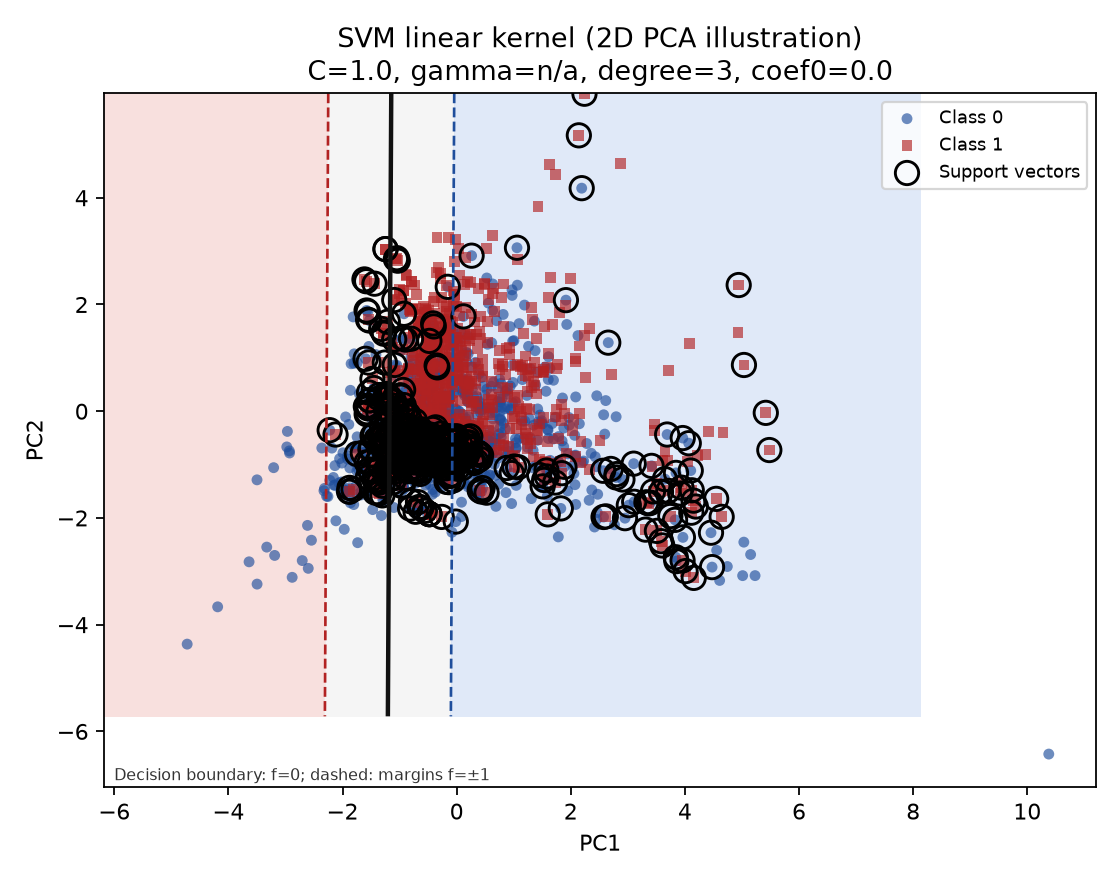
\includegraphics[width=\linewidth]{assets/svm/svm-margin-linear.png}\\
    (a) Linear
  \end{minipage}\hfill
  \begin{minipage}{0.32\textwidth}
    \centering
    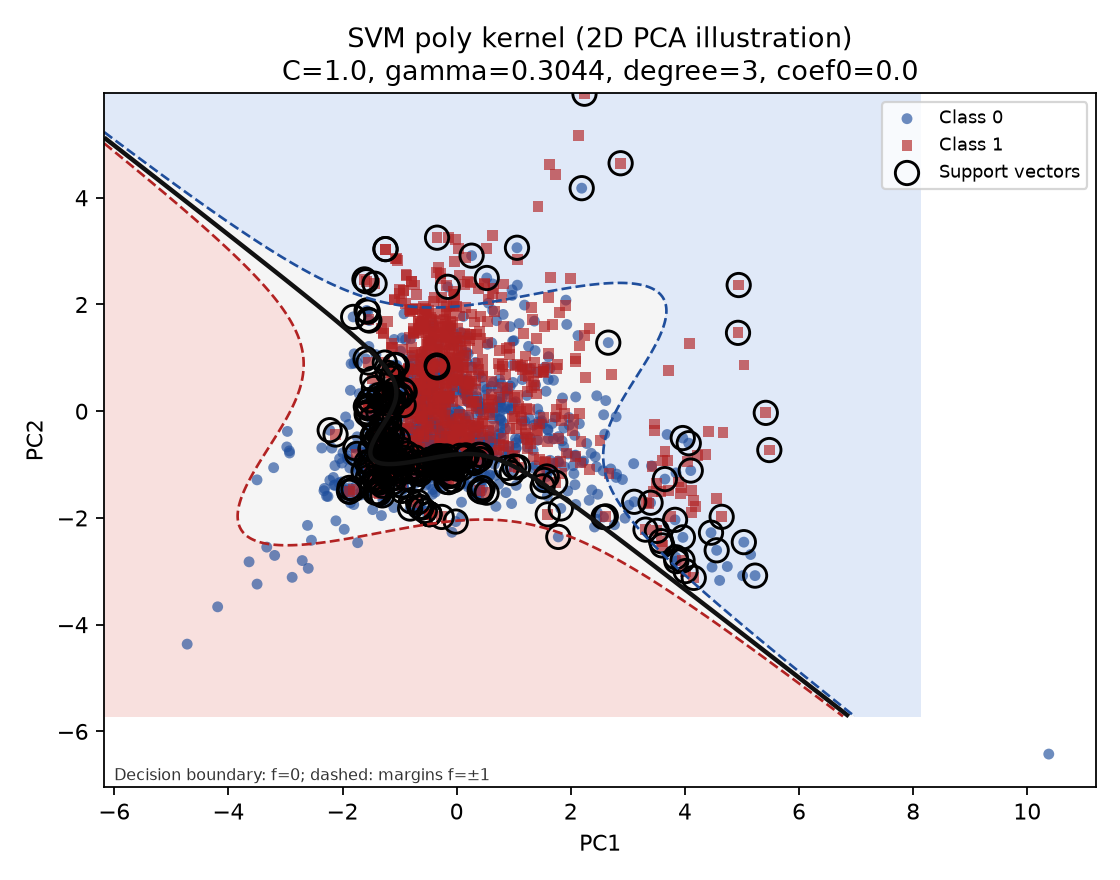
\includegraphics[width=\linewidth]{assets/svm/svm-margin-poly.png}\\
    (b) Polinomial ($d=3$)
  \end{minipage}\hfill
  \begin{minipage}{0.32\textwidth}
    \centering
    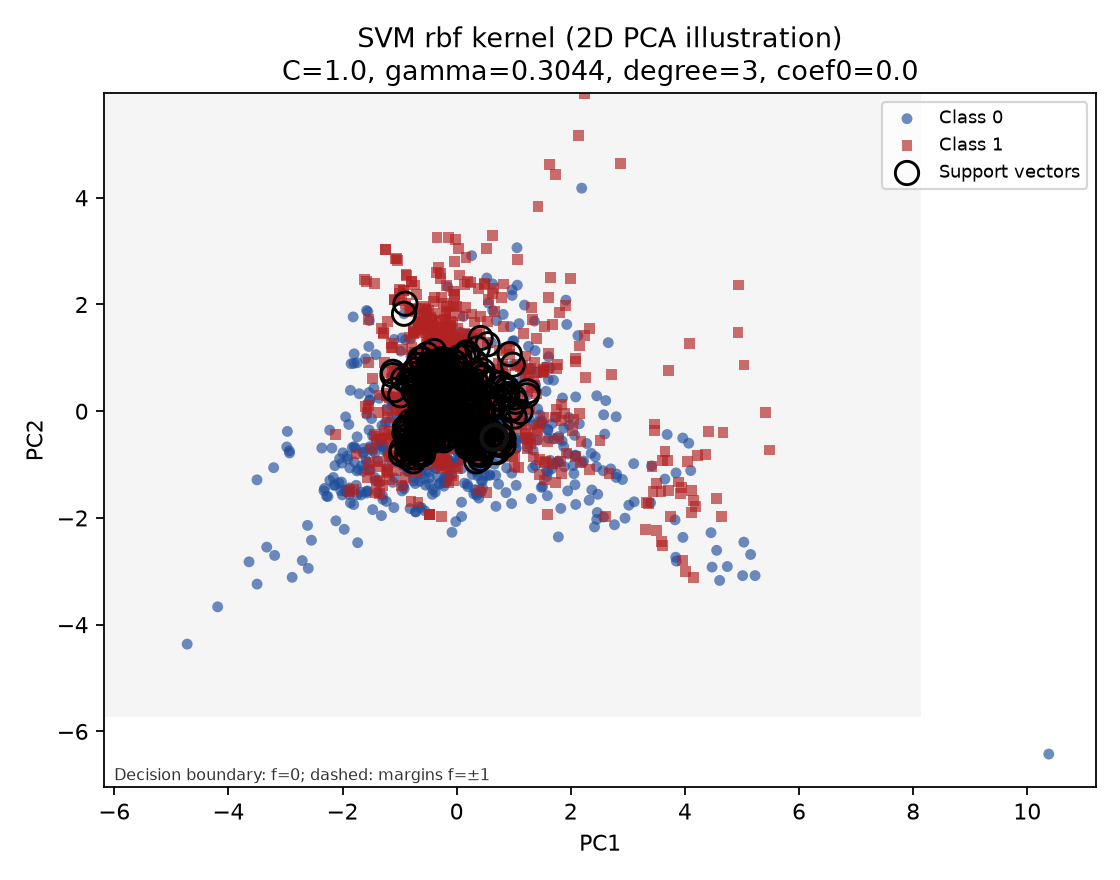
\includegraphics[width=\linewidth]{assets/svm/svm-margin-rbf.png}\\
    (c) RBF
  \end{minipage}
  \caption{Ilustrasi batas keputusan dan \textit{margin} SVM pada dua komponen
  utama pertama. Garis hitam adalah $f(x)=0$, garis putus-putus adalah
  \textit{margin} $f(x)=\pm 1$, dan lingkaran hitam menandai \textit{support
  vector}.}
  \label{fig:svm-margin}
\end{figure}

Peningkatan terbesar justru datang dari rekayasa fitur, bukan dari pemilihan
\textit{solver}. Tabel~\ref{tab:svm-engineered} menunjukkan bahwa dengan 89
fitur hasil rekayasa (interaksi tanggal, rasio harga, target encoding
terhalus, dan indikator nilai hilang) serta penskalaan \textit{robust}, akurasi
naik dari kisaran 0,75--0,77 menjadi 0,8363 pada 5.000 baris dan 0,8500 pada
10.000 baris ($C=15$, RBF). Pada kedua konfigurasi, metrik \textit{from
scratch} dan scikit-learn kembali sama hingga empat angka desimal, dengan
jumlah \textit{support vector} yang berbeda paling banyak satu.

\begin{table}[htbp]
  \centering
  \caption{Hasil SVM RBF pada fitur hasil rekayasa (89 fitur, $C=15$,
  $\gamma=$ \texttt{scale}). Nilai scikit-learn identik hingga empat angka
  desimal.}
  \label{tab:svm-engineered}
  \footnotesize
  \begin{tabular}{lcccccc}
    \toprule
    Konfigurasi & $n$ latih & Akurasi & Macro-F1 & F1 kelas 1 & SV & Latih (s) \\
    \midrule
    Rekayasa fitur & 5.000  & 0,8363 & 0,8104 & 0,7403 & 2123 & 10,21 \\
    Rekayasa fitur & 10.000 & 0,8500 & 0,8261 & 0,7617 & 4140 & 50,09 \\
    \bottomrule
  \end{tabular}
\end{table}

Konfigurasi final untuk submisi menggunakan kernel RBF, fitur hasil rekayasa,
target encoding yang diperluas (116 fitur), dan penyetelan ambang keputusan.
Tiga konfigurasi yang diuji dirangkum pada Tabel~\ref{tab:svm-final}. Model
murni SVM dengan 89 fitur, $C=20$, dan $\gamma = 1{,}25/(d\cdot\mathrm{Var}(X))$
memberikan skor publik terbaik, yaitu 0,86363, dengan akurasi \textit{holdout}
0,8618 (0,8635 setelah ambang disetel ke 0,0695), \textit{macro-F1} 0,8387, dan
AUC 0,9158. Varian \textit{compliant} dengan target encoding diperluas (116
fitur, $C=10$, 22.000 baris) memberikan rata-rata akurasi validasi silang
5-\textit{fold} 0,8642 (0,8645 pada ambang terbaik), \textit{macro-F1} 0,8435,
dan AUC 0,9176; model ini konvergen dengan 8.147 \textit{support vector} dan
KKT $9{,}97\times10^{-4}$ dalam waktu latih sekitar 200 detik. Varian dengan
fitur KNN mencapai \textit{holdout} tertinggi (0,8846) dan AUC 0,9274, tetapi
karena memakai keluaran model lain sebagai fitur (mendekati \textit{stacking}),
varian tersebut hanya dipakai sebagai eksperimen, bukan submisi SVM murni.

\begin{table}[htbp]
  \centering
  \caption{Ringkasan konfigurasi SVM final dan performanya. Skor publik adalah
  akurasi pada data uji Kaggle.}
  \label{tab:svm-final}
  \footnotesize
  \resizebox{\textwidth}{!}{%
  \begin{tabular}{lccccccc}
    \toprule
    Konfigurasi & $n$ & Fitur & $C$ & Akurasi & Macro-F1 & AUC & Publik \\
    \midrule
    SVM murni (submisi terbaik) & 15.000 & 89  & 20 & 0,8618$^{*}$ & 0,8387 & 0,9158 & 0,86363 \\
    SVM + target encoding       & 22.000 & 116 & 10 & 0,8642$^{\dagger}$ & 0,8435 & 0,9176 & -- \\
    SVM + fitur KNN (eksperimen) & 15.000 & 97 & 20 & 0,8846$^{*}$ & 0,8664 & 0,9274 & 0,86300 \\
    \bottomrule
  \end{tabular}}
  \par\vspace{2pt}
  {\scriptsize $^{*}$akurasi \textit{holdout}; $^{\dagger}$rata-rata akurasi
  validasi silang 5-\textit{fold}.}
\end{table}

\paragraph{Reproduksibilitas.}
Seluruh eksperimen dapat dijalankan ulang melalui
\texttt{scripts/run\_svm\_experiments.py} (perbandingan tiga kernel),
\texttt{scripts/train\_final\_scratch.py} (model murni SVM),
\texttt{scripts/train\_final\_compliant\_svm.py} (varian \textit{compliant}),
dan \texttt{scripts/train\_single\_knn\_svm.py} (varian fitur KNN). Metrik
mentah tersimpan pada \texttt{artefacts/svm\_metrics.csv},
\texttt{artefacts/svm\_timing.json}, \texttt{artefacts/scratch\_final\_15k/metrics.json},
dan \texttt{artefacts/compliant\_svm/metrics.json}, sedangkan model serta berkas
submisi tersimpan pada direktori \texttt{output/}.

\paragraph{Analisis beban komputasi.}
Kompleksitas waktu SVM bergantung pada jumlah baris latih $n$ dan jumlah
\textit{support vector}. Pembangunan matriks kernel membutuhkan $O(n^2)$
elemen, sehingga penggunaan memori menjadi kendala utama. Pada perbandingan
5.000 baris, latihan \textit{from scratch} 5--17 kali lebih lambat daripada
scikit-learn (yang memakai kode C yang telah dioptimalkan), tetapi waktu
prediksi kedua implementasi sebanding. Ketika jumlah data dan \textit{cache}
diperbesar, biaya latih meningkat tajam: konfigurasi 10.000 baris dengan
\textit{cache} 512 MB memerlukan sekitar 435 detik karena baris kernel harus
dihitung ulang, sedangkan konfigurasi final 22.000 baris dengan
\textit{cache} 5 GB yang menampung seluruh matriks kernel selesai dalam
sekitar 200 detik. Karena itu, pemilihan ukuran subset dan \textit{budget}
\textit{cache} merupakan kompromi penting antara akurasi dan waktu.

\paragraph{Analisis kesalahan dan keterbatasan.}
Pada \textit{confusion matrix} kernel RBF (subset 5.000 baris), dari 2.741
baris negatif, 2.186 terklasifikasi benar dan 555 menjadi \textit{false
positive}; dari 1.340 baris positif, 951 benar dan 389 menjadi \textit{false
negative}. Artinya model cenderung lebih sering memprediksi pembatalan
(\textit{recall} kelas positif 0,7097) dengan \textit{precision} 0,6315.
Ketidakseimbangan kelas (32,77\% positif) dan tumpang tindih antar kelas
menjadi penyebab utama. Penyetelan ambang keputusan membantu menyelaraskan
laju prediksi positif dengan laju kelas positif sebenarnya (sekitar 29,5\%).
Keterbatasan lain adalah SVM hanya mendukung klasifikasi biner (cukup untuk
dataset ini), biaya $O(n^2)$ membatasi penggunaan seluruh data latih, dan hasil
sangat bergantung pada penskalaan fitur serta pemilihan $\gamma$. Secara
keseluruhan, implementasi \textit{from scratch} terbukti benar karena mampu
mereproduksi perilaku scikit-learn hampir persis, baik dari sisi metrik maupun
skor keputusan.
